\begin{frame}{\insertsubsection}
  \center%
  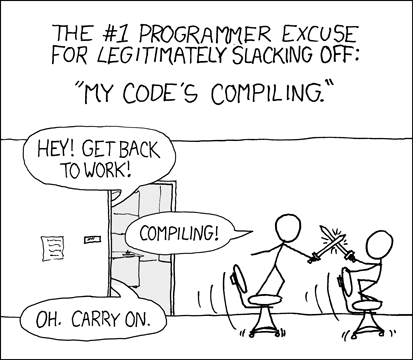
\includegraphics[height = .8\textheight]{compiling.png}

  \note{

    \textbf{Медленное время компиляции} в Rust обусловлено тем, что
    \textbf{атомарной единицей} компиляции является не один файл (как в C/C++),
    а \textbf{целый crate} (или библиотека).

    Вопрос сейчас решается, уже разработано несколько уровней
    \textbf{промежуточного представления}, позволяющих проводить
    \textbf{инкрементную компиляцию}, существуют инструменты \textbf{кэширования
      промежуточных состояний} компиляции. К тому же в cargo встроена
    возможность \textbf{проверки кода на ошибки}, которая отрабатывает очень
    быстро, в IDE ошибки отображаются сразу же.

  }
\end{frame}